% !TEX TS-program = pdflatex
% !TEX encoding = UTF-8 Unicode

% This is a simple template for a LaTeX document using the "article" class.
% See "book", "report", "letter" for other types of document.

\documentclass[11pt]{article} % use larger type; default would be 10pt

\usepackage[utf8]{inputenc} % set input encoding (not needed with XeLaTeX)

%%% Examples of Article customizations
% These packages are optional, depending whether you want the features they provide.
% See the LaTeX Companion or other references for full information.

%%% PAGE DIMENSIONS
\usepackage{geometry} % to change the page dimensions
\geometry{a4paper} % or letterpaper (US) or a5paper or....
% \geometry{margin=2in} % for example, change the margins to 2 inches all round
% \geometry{landscape} % set up the page for landscape
%   read geometry.pdf for detailed page layout information
\addtolength{\topmargin}{-1in}
\addtolength{\textheight}{2in}

\usepackage{graphicx} % support the \includegraphics command and options

% \usepackage[parfill]{parskip} % Activate to begin paragraphs with an empty line rather than an indent

%%% PACKAGES
\usepackage{booktabs} % for much better looking tables
\usepackage{array} % for better arrays (eg matrices) in maths
\usepackage{paralist} % very flexible & customisable lists (eg. enumerate/itemize, etc.)
\usepackage{verbatim} % adds environment for commenting out blocks of text & for better verbatim
\usepackage{subfig} % make it possible to include more than one captioned figure/table in a single float
% These packages are all incorporated in the memoir class to one degree or another...

%%% HEADERS & FOOTERS
\usepackage{fancyhdr} % This should be set AFTER setting up the page geometry
\pagestyle{fancy} % options: empty , plain , fancy
\renewcommand{\headrulewidth}{0pt} % customise the layout...
\lhead{}\chead{}\rhead{}
\lfoot{}\cfoot{\thepage}\rfoot{}

%%% SECTION TITLE APPEARANCE
\usepackage{sectsty}
\allsectionsfont{\sffamily\mdseries\upshape} % (See the fntguide.pdf for font help)
% (This matches ConTeXt defaults)

%%% ToC (table of contents) APPEARANCE
\usepackage[nottoc,notlof,notlot]{tocbibind} % Put the bibliography in the ToC
\usepackage[titles,subfigure]{tocloft} % Alter the style of the Table of Contents
\renewcommand{\cftsecfont}{\rmfamily\mdseries\upshape}
\renewcommand{\cftsecpagefont}{\rmfamily\mdseries\upshape} % No bold!

%%% END Article customizations

\newcommand\tag[1]{\texttt{#1}}

%%% The "real" document content comes below...

\title{PROTEST: Manual Annotation Guidelines\\Version 1.0}
%\author{The Author}
%/\date{9 February 2016} % Activate to display a given date or no date (if empty),
         % otherwise the current date is printed 

\begin{document}
\maketitle

\section{Introduction}
\textit{PROTEST} is a pronoun test suite, designed to enable researchers to evaluate their Machine Translation (MT) systems on the specific task of pronoun translation. The test suite comprises:
\begin{itemize}
  \item 250 hand-selected pronoun tokens, categorised according to a number of features
  \item An automatic evaluation script
  \item A graphical user interface (GUI), which may be used to:
  \begin{itemize}
    \item Browse the translations of the set of hand-selected pronoun tokens
    \item Manually annotate pronoun tokens that cannot be evaluated automatically
  \end{itemize}
\end{itemize}

\section{Getting started}
To run the PROTEST manual annotation tool:
\begin{enumerate}
  \item Open a terminal window
  \item Navigate to the PROTEST directory
  \item Run the command: \textbf{sh gui.sh}
\end{enumerate}

\noindent
This will open the \textbf{Database Selection window} (see Figure \ref{fig:DatabaseWindow}).

\begin{figure}[h!]
    \centering
    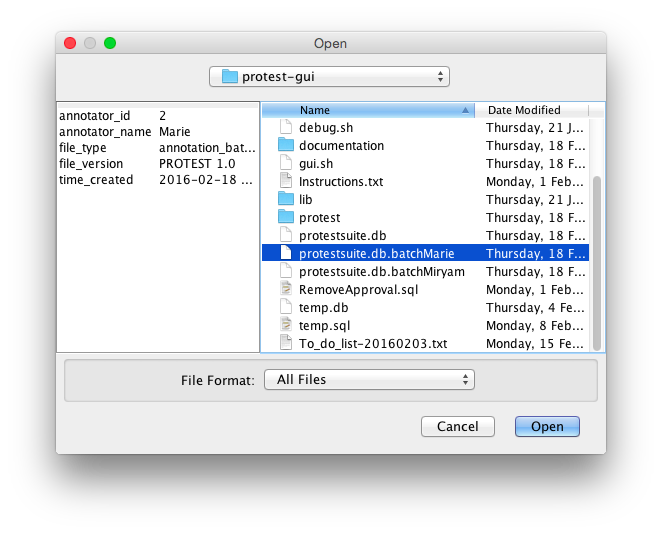
\includegraphics[width=0.60\textwidth]{DatabaseSelectionWindow.png}
    \caption{Database Selection window}
    \label{fig:DatabaseWindow}
\end{figure}

Browse to and select the database that contains the annotation task that you wish to work on. Click on the \textbf{Open} button.

The \textbf{Batch Selection window} will open (see Figure \ref{fig:BatchWindow}). The \textbf{Batch Selection window} displays a list of pronoun categories and a set of buttons for each:

\begin{itemize}
  \item New: unannotated pronouns
  \item Done: annotated pronouns
  \item Conflict: pronouns for which the annotations are conflicting (see Section \ref{ConflictingAnnotations})
\end{itemize}

\begin{figure}[h!]
    \centering
    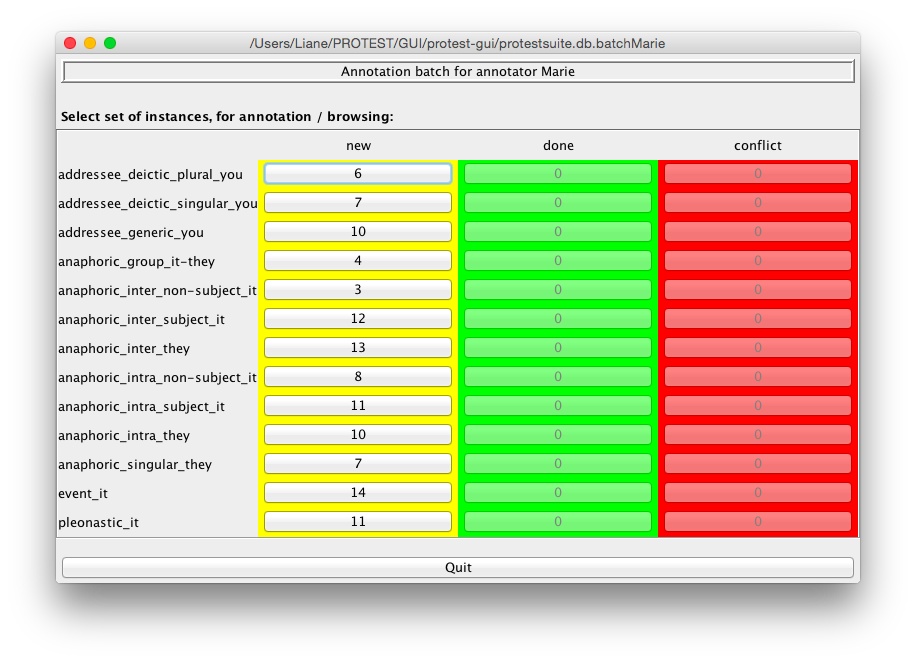
\includegraphics[width=0.85\textwidth]{BatchSelectionWindow.png}
    \caption{Batch Selection window}
    \label{fig:BatchWindow}
\end{figure}

Select the batch that you wish to annotate or review and click on the relevant button. This will open the \textbf{Manual Annotation window} (see Figure \ref{fig:AnnotationWindow}).

\begin{figure}[h!]
    \centering
    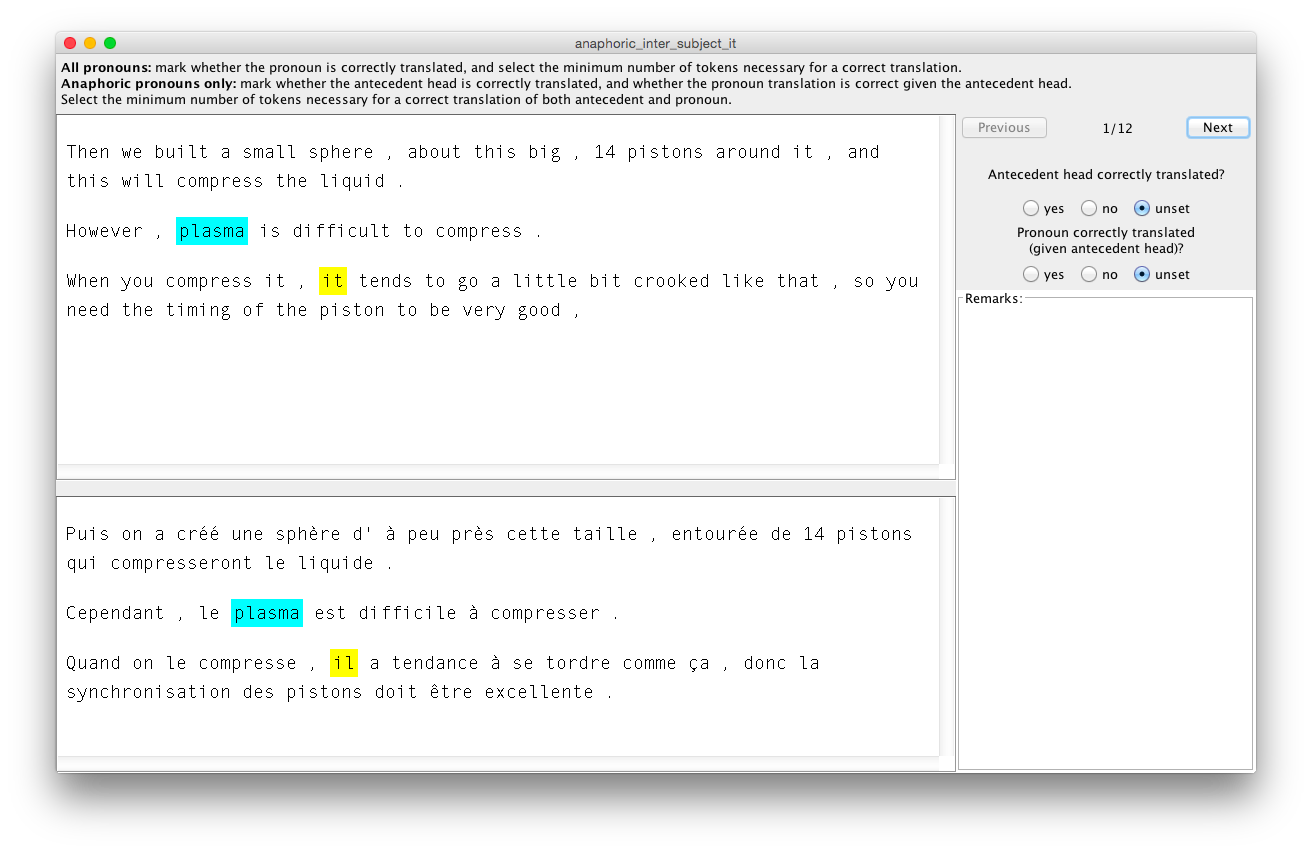
\includegraphics[width=0.99\textwidth]{ManualAnnotationWindow.png}
    \caption{Manual Annotation window}
    \label{fig:AnnotationWindow}
\end{figure}

Follow the annotation guidelines in Section \ref{AnnotationGuidelines} to complete the annotations. Your annotations will be saved automatically when you use the \textbf{Previous} and \textbf{Next} buttons to navigate between pronoun tokens in the set, or when you close the \textbf{Manual Annotation window}.

To exit the PROTEST manual annotation tool, click on the \textbf{Quit} button in the \textbf{Batch Selection window}.


\section{Annotation Task Overview}
The aim of the annotation task is to assess the ability of MT systems to translate pronouns, and to create a corpus of acceptable translations of pronouns.

For each example you are shown, you will be asked to provide the following information:
\begin{itemize}
\item\emph{Overall assessment:} Decide whether or not the pronoun is translated
	correctly. In the case of anaphoric pronouns, you will also be asked to
	assess the translation of the pronoun's antecedent head.
\item\emph{Token selection:} For those translations marked as ``correct'', you
	will also be asked to select the minimum set of tokens that constitute
	a correct translation.
\item\emph{Tags:} We ask you to mark certain recurring patterns in the examples
	by assigning \emph{tags}. A standard set of tags for common problems is
	described in section~\ref{Tags}. You may also create new tags if you spot
	other types of recurring patterns. Try to use them as consistently as
	possible.
\item\emph{Remarks:} You also have the possibility to add free-text remarks to the examples.
	Please use this function to record any information that may be useful in
	the use or evaluation of the annotations. You might for instance want to add
	explanatory notes if you are unsure about the annotation of an example, or if
	you had to make certain assumptions about the interpretation of the text.
\end{itemize}

In this annotation task, we focus on the correctness of the highlighted
pronouns and their antecedents. We are not interested in the correctness of the
other words in the translated sentences, except where this makes it impossible
to assess the correctness of the pronoun and antecedent head translations.

Please familiarise yourself with the annotation guidelines before starting the annotation task.

\section{Annotation Guidelines}
\label{AnnotationGuidelines}
Select a batch of pronoun tokens from the \textbf{Batch Selection window}, for the desired MT system and pronoun category. The \textbf{Manual Annotation window} will appear. For each highlighted pronoun token, read the source-language text (top frame) and the MT system output (bottom frame). Please note that you may need to use the scroll bars on the right-hand side of the text boxes to read the complete source text and translation. Consider the translation of the source-language pronoun token that is highlighted in yellow. If the source-language pronoun was translated by the MT system, the translation (consisting of one or more tokens) in the MT system output will also be highlighted in yellow.

Complete the annotation of each pronoun instance using the following guidelines:


\subsection{General Guidelines: All Pronouns}

\begin{itemize}
  \item Answer the question: ``Pronoun Correctly Translated?'' using the ``yes/no'' options in the \textbf{annotation panel} in the top right-hand corner of the \textbf{Manual Annotation window}
  \begin{itemize}
    \item You should answer this question for all source-language pronouns, whether or not they are translated by the MT system
    \item As the aim of the annotation task is to produce a corpus of acceptable translations for use in automatic evaluation, we place a higher value on precision. This means that you should only mark translations as correct if you feel that it is something ``natural'' that you might say yourself, or that you might expect to hear someone else say. The only exception to this rule is for the annotation of deictic, singular addressee reference pronouns, where we consider both formal and informal (``vous'' and ``tu'') to be valid translations of deictic singular ``you'' (see Section \ref{AddresseeGuidelines})
    \item If the pronoun is translated according to something that a French speaker might (naturally) say but French grammar rules would disagree, add the \tag{desc\_vs\_presc} to the \textbf{tags list}
    \item If a source-language pronoun is left untranslated by the MT system, use the ``yes/no'' options to mark whether this is correct/incorrect.
    \item If you are unsure because something looks to be ``unusual'', it is best to mark the translation as incorrect, and add the relevant tag to indicate what you are unsure about. More information on the use of tags is included in Section \ref{Tags}. Please also use the \textbf{remarks box} on the right-hand side of the \textbf{Manual Annotation window} to record any notes that you believe may be useful later on.
    \item You may come across badly translated sentences, with some translated so badly that you cannot understand their meaning. If you believe that it is possible to assess the translation of the pronoun independently of the remainder of the translation output, you should annotate the example as normal. If not, you should leave the example un-annotated, add the \tag{bad\_translation} tag, and (optionally) a comment in the \textbf{remarks box}.
    \item If the pronoun is present in the translation output but appears outside of the yellow highlighted tokens (i.e. a bad alignment), do not attempt to annotate the example. Instead, add the \tag{incorrect\_word\_alignment} tag to the \textbf{tags list}, and (optionally) a comment in the \textbf{remarks box}. (Note: The \tag{incorrect\_word\_alignment} tag must not be used if the pronoun translation appears within the set of yellow highlighted tokens.)
    \item You may come across pronoun translations were the pronoun is part of a fixed phrase which cannot be decomposed in such a way that the pronoun in the translation is considered to mean the same thing as the pronoun in the source language text. For example if an event reference ``it'' is translated as ``if faut'' in French. In cases such as these:
    	\begin{itemize}
		\item Add the \tag{noncompositional\_translation} tag to the \textbf{tags list}
		\item Consider not only the translation of the pronoun, but of the clause that contains the pronoun (or whatever unit you consider to be relevant)
		\item \textit{If the translation of the clause is acceptable:} mark the pronoun translation as correct but do not select any tokens
	\end{itemize}
    \item Note: if the pronoun is anaphoric, follow the guidelines in Section \ref{AnaphoricGuidelines}
    \item Note: if the pronoun is deictic, singular, addressee reference, you should also add a politeness tag. See Section \ref{AddresseeGuidelines} for details
  \end{itemize}
  \item \textit{If you have marked the pronoun translation as correct:} Select the \textit{minimum} number of yellow highlighted tokens that constitutes a correct translation of the source-language pronoun. To select a token, click on it. The token highlight will change to orange, indicating that it has been selected. You can select as many highlighted tokens as are required. It is not possible to select tokens that do not have a yellow highlight.
  \item Please use the \textbf{remarks box} to record any issues that you would like to discuss, e.g. relating to any difficulties that you encounter or uncertainties that you may have, during the annotation of a given pronoun.
  \item Once you have completed the annotation of the current pronoun instance, move to the next one using the \textbf{Next} button in the top right hand corner of the \textbf{Manual Annotation window}
  \begin{itemize}
    \item If the annotations are conflicting, for example if you have indicated that the pronoun is correctly translated but none of the translated tokens has been selected, a warning will appear. You may choose to make a correction, or proceed to the next pronoun instance.
  \end{itemize}
\end{itemize}

\subsection{Deictic, Singular, Addressee reference Pronouns}
\label{AddresseeGuidelines}
A politeness tag should be added for every example of a deictic, singular addressee reference pronoun, regardless of whether its translation is deemed correct or not.

For singular, deictic addressee reference pronouns (i.e., ``you'' referring to
a single person), French distinguishes two levels of formality/politeness,
``tu'' and ``vous''. We ignore this distinction in the \emph{overall
assessment},  so pronouns where ``tu'' would have been more appropriate
than ``vous'' (and vice versa) should be labelled as correctly translated.
However, for this class of pronouns, the appropriate level of politeness should
be marked. This is achieved by inserting the relevant tag in the \textbf{tags list} on the
right-hand side of the \textbf{Manual Annotation window}. Please select from the following tags:
\tag{politeness\_tu}, \tag{politeness\_vous} and \tag{politeness\_unknown}.
The latter tag should be used if the context doesn't give you enough information
to decide whether ``tu'' or ``vous'' would be preferable.

When choosing between levels of formality, consider first and foremost which of
the forms you yourself would be likely to use in a given context, or, failing
that, which form the average modern French speaker would be likely to use. We
recognise that the use of formality markers may be a bit different in specific
(e.g., very conservative or very progressive) communities. Here, we ask you to
make choices that, in your opinion, the majority of French speakers would
consider normal. If in doubt, select the
\tag{politeness\_unknown} tag.

\subsection{Anaphoric Pronouns Only}
\label{AnaphoricGuidelines}

If the pronoun is anaphoric, you will need to consider both the translation of the antecedent head and the pronoun. The \textit{head} of the source-language pronoun's \textit{antecedent} will be highlighted in light blue. If the antecedent head has been translated by the MT system, the translation (consisting of one or more tokens) in the MT system output will also be highlighted in light blue.

\begin{itemize}
  \item First, answer the question: ``Antecedent Correctly Translated?'' using the ``yes/no'' options in the \textbf{annotation panel} in the top right-hand corner of the \textbf{Manual Annotation window}
  \begin{itemize}
    \item Antecedent heads have been manually labelled and should therefore be correct in the majority of cases. However, if you believe that the antecedent head choice is incorrect, please add the \tag{ant\_unsure} tag to the \textbf{tags list}
    \item If the pronoun or the antecedent head are present in the translation output but is not highlighted (i.e. a bad alignment), do not attempt to annotate the example. Instead, add the \tag{incorrect\_word\_alignment} tag to the \textbf{tags list}
  \end{itemize}  
  \item \textit{If you have marked the antecedent head translation as correct:} Select the \textit{minimum} number of blue highlighted tokens that constitutes a correct translation of the source-language antecedent head. Note that we are interested in noun tokens, not articles or punctuation etc. To select a token, click on it. The token highlight will change to a darker shad of blue, indicating that it has been selected. You can select as many highlighted tokens as are required. It is not possible to select tokens that do not have a blue highlight
  \item Second, answer the question: ``Pronoun Correctly Translated (given antecedent head)?'' using the ``yes/no'' options in the \textbf{annotation panel}
  \begin{itemize}
    \item A correctly translated pronoun is one that is \textit{compatible}
	    with the translation of the antecedent head, regardless of whether
	    the antecedent head is translated correctly. Compatibility
	    frequently coincides with the notion of morphosyntactic agreement,
	    but it does not always do so. An example of a compatible
	    pronoun-antecedent pair violating morphosyntactic agreement is the
	    use of ``singular they'' in English to refer to a single person --
	    formally, the pronoun ``they'' is a plural and does not agree in
	    number with its antecedent, but the use of ``they'' to refer to
	    singular antecedents is acceptable in English (for example in the
	    case where the gender of the person is unknown) and should
	    therefore be marked as correct.
  \end{itemize}
  \item \textit{If you have marked the pronoun translation as correct:} Select the \textit{minimum} number of yellow highlighted tokens that constitutes a correct translation of the source-language pronoun (given the antecedent head)
\end{itemize}


\section{Annotation Tags}
\label{Tags}
Tags are used to denote specific recurring patterns, where errors may be present.

The following tags may be entered into the \textbf{tags list} for any pronoun category:

\begin{itemize}
  \item \tag{ant\_unsure}: Unsure if antecedent has been correctly identified in English source sentence.
  \item \tag{bad\_translation}: Overall sentence translation is so poor that it is not possible to judge whether the translation of the pronoun/antecedent is correct.
  \item \tag{noncompositional\_translation}: Used when the pronouns have different functions in the two languages. For example, if an English event pronoun is translated as ``il faut'' (a fixed expression where ``il'' is a pleonastic pronoun), the English pronoun cannot be said to be translated as ``il''
  \item \tag{incorrect\_word\_alignment}: Pronoun/antecedent translation exists in the translation of the source-language text but has not been highlighted due to a problem with the word alignments
  \item \tag{desc\_vs\_presc}: Signals a conflict between something that a French speaker might (naturally) say and what French grammar rules state.
\end{itemize}  

The following tags should be used for the addressee reference, deictic, singular pronouns category only:

\begin{itemize}  
  \item \tag{politeness\_tu}: You are sure that the pronoun should be ``tu''
  \item \tag{politeness\_vous}: You are sure that the pronoun should be ``vous''
  \item \tag{politeness\_unknown}: You are unable to tell whether the pronoun should be ``tu'' or ``vous'' given the available context
\end{itemize}


\section{Conflicting Annotations}
\label{ConflictingAnnotations}
There are a number of scenarios which give rise to warnings about conflicting annotations:
\begin{itemize}
  \item All pronouns:
  \begin{itemize}
    \item Pronoun is marked as correct, but no tokens are selected in the translation output
    \item Tokens are selected in the translation of the pronoun, but the pronoun is not marked as correct
    \item Example is marked with the \tag{bad\_translation} tag but annotations are provided
    \item Example is marked with the \tag{incorrect\_word\_alignment} tag but annotations are provided
    \item Pronoun translation is marked with the \tag{noncompositional\_translation} tag but tokens are selected
    \item Example is marked with more than one of the three tags \tag{bad\_translation}, \tag{incorrect\_word\_alignment} and \tag{noncompositional\_translation}
  \end{itemize}
  \item Anaphoric pronouns only:
  \begin{itemize}
    \item Antecedent is marked as correct, but no tokens are selected in the translation output
    \item Tokens are selected in the translation of the antecedent head, but the antecedent head is not marked as correct 
  \end{itemize}
\end{itemize}

In the case of anaphoric pronouns, conflicts may exist in the annotation of the pronoun, its antecedent head, or both.


\end{document}
